%!TEX root=Principal.tex
\chapter{TECNOLOGIAS E TESTES}
\label{cap:tecnologiaetestes}
Esse capítulo apresentará as tecnologias e equipamentos utilizados para o desenvolvimento e o cenário de teste considerado para validação do processo de interação entre humanos e robôs proposto por essa tese.

\section{O Robô}
\label{sec:robo}
O robô utilizado no desenvolvimento da tese é o PeopleBot~\footnote{PeopleBot - http://www.mobilerobots.com/researchRobots/PeopleBot.aspx} fabricado pela ActivMedia Robotics. Ele é um robô móvel com direção diferencial, ou seja, possui duas rodas motorizadas e uma roda castor que auxilia em seu equilíbrio. O projeto do PeopleBot tem foco em pesquisas e serviços que envolvem interação humano-robô. Com esse objetivo, ele foi desenvolvido com uma altura de 112 cm (centímetros). Além disso, o PeopleBot também possui uma garra pequena que tem sua movimentação apenas na direção vertical. A figura~\ref{fig:peoplebot} apresenta o robô PeopleBot.

\begin{figure}[ht!]
	\centering
	\begin{minipage}{\textwidth}
		\caption{Robô ActivMedia Robotics PeopleBot.}
		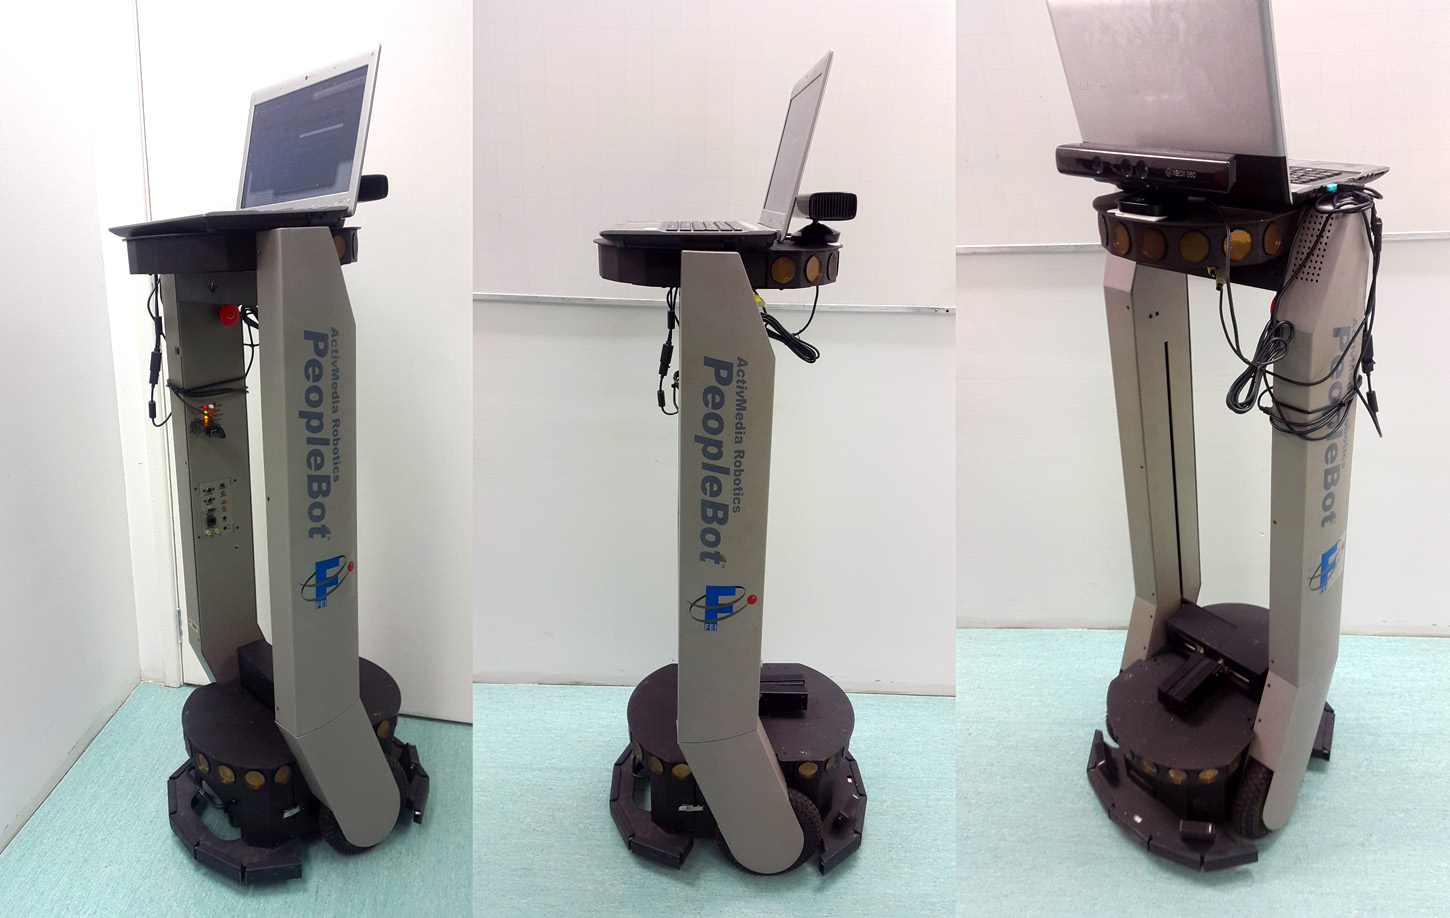
\includegraphics[width=\textwidth]{peoplebot.jpg}
		\smallcaption{Fonte: Autor.}
		\label{fig:peoplebot}
	\end{minipage}
\end{figure}

Como a garra do PeopleBot é curta e não permite muita destreza na manipulação de objetos e gestos, além de possuir poucos graus de liberdade, foi adicionado um novo manipulador. O projeto do manipulador foi desenvolvido com o intuito de auxiliar a manipulação de objetos a uma certa distância e execução de gestos durante interações com pessoas. O projeto atende pesquisas com foco em prestação de serviços domésticos e cuidados pessoais. O desenho que ilustra o manipulador desenvolvido é apresentado através da figura~\ref{fig:manipulador}.

\begin{figure}[ht!]
	\centering
	\begin{minipage}{0.6\textwidth}
		\caption{Projeto do Novo Manipulador do PeopleBot.}
		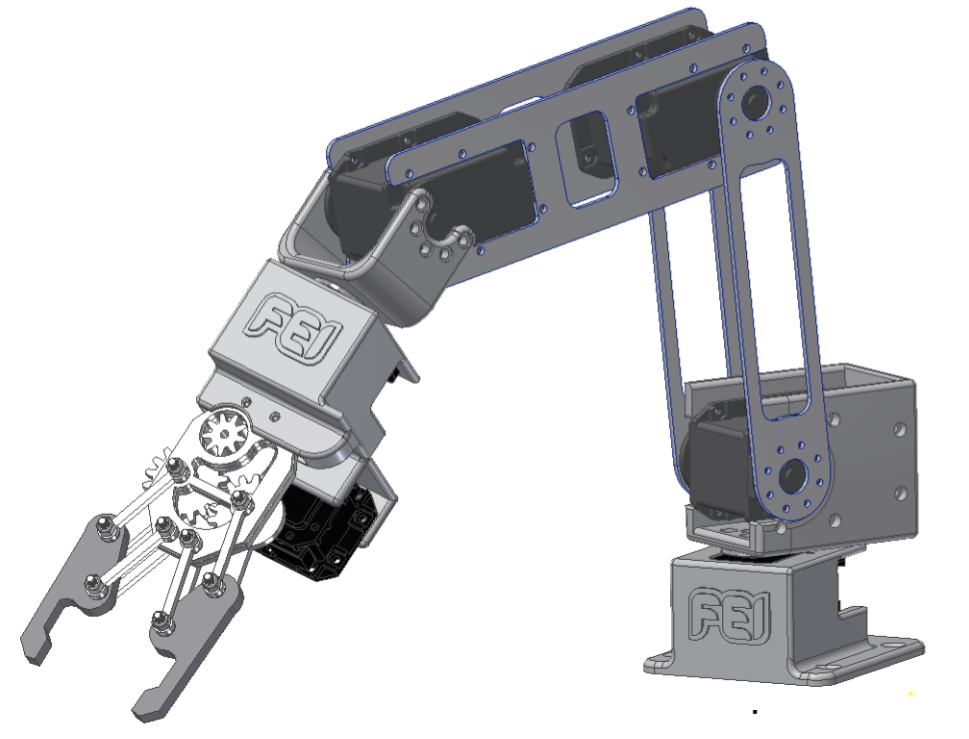
\includegraphics[width=\textwidth]{manipulador.png}
		\smallcaption{Fonte: Autor.}
		\label{fig:manipulador}
	\end{minipage}
\end{figure}

O novo manipulador foi construído de maneira que os movimentos sejam próximos do braço humano. Além do manipulador, também foi acoplado um \emph{tablet} para que seja possível atribuir face ao robô e consequentemente expressões faciais, deixando a interação mais amigável. O projeto da cabeça do robô é apresentado na figura~\ref{fig:judithhead}.

\begin{figure}[ht!]
	\centering
	\begin{minipage}{0.4\textwidth}
		\caption{Projeto da Cabeça para o PeopleBot.}
		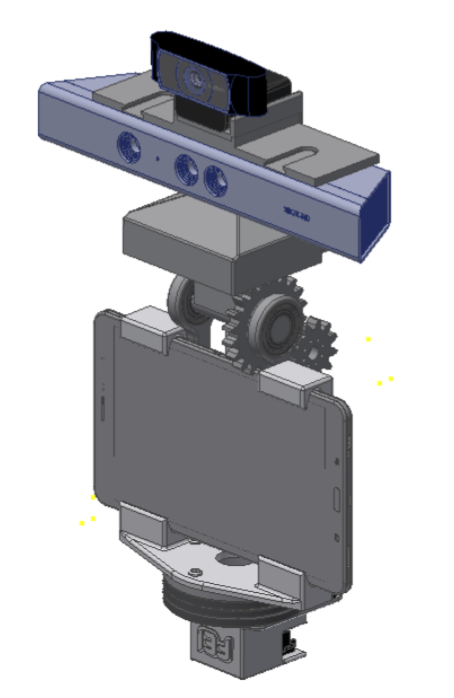
\includegraphics[width=\textwidth]{judith_head.png}
		\smallcaption{Fonte: Autor.}
		\label{fig:judithhead}
	\end{minipage}
\end{figure}

O projeto da cabeça foi preparado para acomplar alguns alguns sensores como o Microsoft\textregistered\ Kinect\textregistered\ , o ASUS\textregistered\ Xtion\textregistered\ e webcams, para tarefas que envolvam nuvem de pontos de profundidade e visão computacional. Sensores como lasers e microfones também foram instalados para melhorar a captura de informações sobre o ambiente e interagir melhor com a pessoa.

\section{Arquitetura do Software}
\label{sec:arquitetura}
A arquitetura construída para o software do robô foi feita em camadas. Existem 3 camadas principais, que definem a arquitetura do robô. A primeira camada contém os estados que compõem as máquinas de estados que auxiliam o robô nas tarefas a serem realizadas. Basicamente, ela conduz as ações e comandos que o robô tem como interface com o usuário durante a interação.

A segunda camada é responsável pelo processamento dos processos de \emph{subscribers} e \emph{publishers}, conforme o recomendado pelo \emph{Robot Operating System}~(ROS)~\footnote{http://www.ros.org/}. Eles fazem a interface entre sensores e atuadores, através de seus \emph{drivers}, e também com os algoritmos de visão computacional, de aprendizado de máquina e de planejamento. O processamento desses algoritmos, de sensores com grande volume de informação como o Kinect e serviços que auxiliam o controle do manipulador são encontrados na terceira camada.

Como toda a implementação do software foi feita com base no ROS, os pacotes foram construídos de maneira separada. Sendo assim, os códigos fontes ficaram agrupados de acordo com as habilidades necessárias para o robô realizar as tarefas e também referentes ao mesmo tipo de objetivo. Todo o código fonte criado para execução dos testes dessa tese, encontram-se disponível através do endereço \url{https://github.com/amasiero/approach_control}, na ferramente de controle de versão em código aberto, GitHub. O código foi testado com duas bases robóticas, o PeopleBot da Pioneer e o youBot da Kuka.

\subsection{Bibliotecas}
\label{sec:bibliotecas}
Para auxiliar no desenvolvimento da tese, algumas bibliotecas e softwares foram utilizados. O primeiro, conforme dito na seção~\ref{sec:arquitetura}, foi o ROS que é um \emph{framework} para desenvolvimento de software em robôs. Ele roda sobre o Ubuntu Linux, que no caso da tese foi utilizado a versão 14.04, com o ROS versão Indigo.

A biblioteca que gerencia a máquina de estados criada para execução das tarefas é o SMACH~\footnote{http://wiki.ros.org/smach}. Ele possibilita a criação e realiza o gerenciamento dos estados durante a execução das ações do robô. Para reconhecimento de voz a biblioteca utilizada foi o Dragonfly Speech Recognition~\footnote{https://pypi.python.org/pypi/dragonfly/0.6.5}. Bibliotecas como o OpenCV~\footnote{http://opencv.org/}, PyOpenni~\footnote{https://github.com/jmendeth/PyOpenNI} e MoveIt!~\footnote{http://moveit.ros.org/} foram utilizados para percepção e interação com o ambiente e também com o usuário.

Todos os pacotes desenvolvidos utilizaram a linguagem de programação Python, que possibilitou diversas facilidades na implementação dos códigos e integração das camadas dos pacotes no ROS. Para criação e teste da rede bayesiana proposta utilizou-se o \emph{framework} SamIam~\footnote{http://reasoning.cs.ucla.edu/samiam/}, que realiza os cálculos de todas as probabilidades de uma consulta a rede de maneira objetiva e com um bom desempenho computacional.

\section{Cenário de Teste} %REFAZER OS TEXTOS DESSA SEÇÃO
\label{sec:cenario}
Antes de descrever o cenário de teste, é importante mencionar que todo o procedimento para a execução foi aprovado por um comitê de ética, e pode ser consultado a partir do identificador CAAE: 70057117.0.0000.5508. O teste é realizado em um cenário simulando um residência, conforme apresentado na figura~\ref{fig:cenario}. No cenário, o robô irá navegar de maneira autonoma a procura de uma garrafa que ele deixou no armário. Como ele não encontra a garrafa, o robô sai a procura de uma pessoa que esteja na casa para ajuda-lo. Ele irá interagir com a pessoa, e poderá solicitar que a pessoa o siga para algum lugar do cenário, à procura de sua garrafa.

\begin{figure}[ht!]
	\centering
	\begin{minipage}{\textwidth}
		\caption{Cenário para teste de interação com o robô.}
		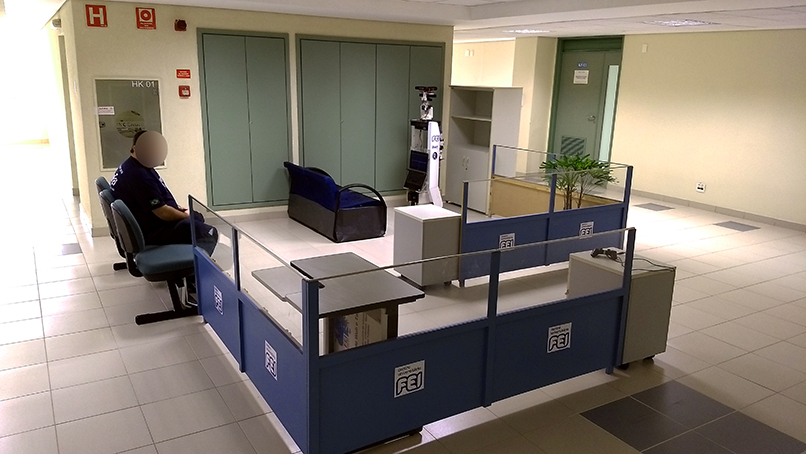
\includegraphics[width=\textwidth]{cenario.jpg}
		\smallcaption{Fonte: Autor.}
		\label{fig:cenario}
	\end{minipage}
\end{figure}

\subsection{Objetivo}

Verificar a compreensão e conforto da pessoa ao observar e interagir com o robô no cenário doméstico, assim identificar experiências positivas e negativas do usuário.

\subsection{Foco}

O foco do cenário é a experiência do usuário com a presença do robô e a interação social entre ambos.

\subsection{Configuração para o Teste}

Para o teste são consideradas algumas possibilidades de posicionamento da pessoa e robô para interagirem.

\begin{itemize}
	\item Pessoa parada em pé e o robô inicia a interação próximo do usuário.
	\item Pessoa parada em pé e o robô inicia a interação distante do usuário.
	\item Pessoa parada sentada e o robô inicia a interação próximo do usuário.
	\item Pessoa parada sentada e o robô inicia a interação distante do usuário.
\end{itemize}

O objetivo das configurações é a aleatoriedade do posicionamento entre robô e pessoa, considerando cenários doméstico onde o convívio é comum. Assim, é possível medir a experiência do usuário em diversas situações de convivência.

\subsection{Tarefa}

Esse teste ocorre em um ambiente controlado, porém o trânsito de outros indíviduos pelo cenário acontece com frequência significativa. O passo a passo da tarefa é descrito na lista a seguir:

\begin{enumerate}
	\item \textbf{Início}: O robô é posicionado no cenário de maneira que esteja em um local em torno da residência simulada.
	\item \textbf{Busca pelo objeto}: O robô segue até uma mesa, ou armário, onde supostamente deixou sua garrafa.
	\item \textbf{Interação com a pessoa}: O robô se aproxima do usuário e questiona se ele viu a garrafa.
	\item \textbf{Nova busca pelo objeto}: O robô segue a um novo ponto em busca da garrafa, que novamente não está no local.
	\item \textbf{Retorno ao usuário}: O robô retorna ao local onde o usuário se encontra e, em uma distância maior ou menor de proximidade (aleatória), solicita que o usuário o acompanhe.
	\item \textbf{Fim}: Será considerado o fim da tarefa, quando o robô alcançar um ponto ao redor do cenário e informar o fim do teste ao participante.
\end{enumerate}

\section{Seleção das Pessoas para o Teste}
\label{sec:perfistestes}
As pessoas possuem idades diversificadas com variedade de 18 a 50 anos. Alguns candidatos ao teste possuem medo declarado de robôs e neste caso o especialista ficará acompanhando o teste com uma maior proximidade para evitar problemas com o robô e principalmente com a pessoa.

São evitados a repetição de configuração entre os candidatos, para que não seja levantado nenhum conhecimento a priori sobre o comportamento do robô.
